%*******************************************************************************
%Modelo de TCC elaborado para o campus Birigui do IFSP. Foram utilizados como referência o pacote ABNTex e os modelos XXXXXXXXXXXX.

%Este trabalho foi realizado dentro do programa de monitoria "Cola comigo que seu TCC fica bonito!".
%Monitor: Gustavo Shoji Nishimura
%Orientador: Prof. Dr. Eduardo Shigueo Hoji

%*******************************************************************************

\documentclass[12pt,oneside,a4paper,chapter=TITLE,section=TITLE,brazil,fleqn,riqno]{abntex2}

\usepackage{./estilo/ifsp}
\DisemulatePackage{setspace}
\usepackage{setspace}

%----------------------------------------------------------------------
%-----------------Informações sobre o autor e a obra ------------------
%----------------------------------------------------------------------
  
\titulo{Título do trabalho}
\def \nomeautor{Eduardo} %Nome do primeiro autor
\def \sobrenomeautor{Mambelli Serotini} %Sobrenome do primeiro autor
\autor{\nomeautor~\sobrenomeautor}
\def \coautor{} %Nome completo do segundo autor. Caso não tenha, deixe em branco entre as chaves.
\def \tercautor{} %Nome completo do terceiro autor. Caso não tenha, deixe em branco entre as chaves.
\local{Piracicaba}
\data{2026}
\orientador{Luís Fernando Lopes Grim}	% Digite o nome do prof. orientador entre as chaves
\coorientador{}	%Caso não possua coorientador, deixar em branco
\instituicao{Instituto Federal de Educação, Ciência e Tecnologia de São Paulo  Câmpus Piracicaba}
\tipotrabalho{Trabalho de Conclusão de Curso }
\preambulo{\imprimirtipotrabalho apresentado ao \imprimirinstituicao, como requisito parcial para conclusão do curso de Engenharia da Computação.} %Escrever no lugar do XXXX o curos no qual o trabalho foi apresentado



%----------------------------------------------------------------------
%-----------------Elementos pré-textuais -----------------------
%----------------------------------------------------------------------
\begin{document}

   
\pretextual
%----------------------------------------------------------------------
%-----------------Inserir a capa no texto -----------------------
%----------------------------------------------------------------------
%\renewcommand{\imprimircapa}{%
\begin{capa}
\center
%\begin{figure}[H]
%	\centering
%	\includegraphics[scale=1]{imagens/logo.png} 
%\end{figure}
%\vspace*{0.5cm}
{\MakeUppercase\imprimirinstituicao}
\vspace*{1.0cm}\\
\textsc{\imprimirautor}\\
\textsc{\coautor}\\
\textsc{\tercautor}
\vfill
\begin{center}
\ABNTEXchapterfont\bfseries\large\MakeUppercase\imprimirtitulo
\\{subtitulo}
\end{center}
\vspace{\fill}
\imprimirlocal\\
\imprimirdata
\vspace*{1cm}
\end{capa}
%}


%----------------------------------------------------------------------
%-----------------Inserir a folha de rosto no texto ------------------
%----------------------------------------------------------------------
\makeatletter
%\renewcommand{\folhaderostocontent}{
\begin{center}
\textsc{\imprimirautor}\\
\textsc{\coautor}\\
\textsc{\tercautor}
\vspace*{\fill}\vspace*{\fill}
\begin{center}
\ABNTEXchapterfont\bfseries\large\MakeUppercase\imprimirtitulo
\\{subtitulo}
\end{center}
\vspace*{\fill}
\abntex@ifnotempty{\imprimirpreambulo}{%
\hspace{.5\textwidth}
\begin{minipage}{.5\textwidth}
\SingleSpacing 
\nohyphens{\imprimirpreambulo}\\\\}
{\bfseries\imprimirorientadorRotulo}{~\nohyphens{\imprimirorientador}\par}
\abntex@ifnotempty{\imprimircoorientador}{%
{\bfseries\imprimircoorientadorRotulo}{~\nohyphens{\imprimircoorientador}}%
}
\end{minipage}%
\vspace*{\fill}

\vspace*{\fill}
\imprimirlocal\\
\imprimirdata
\vspace*{1cm}
\end{center}
%}
\makeatother
%----------------------------------------------------------------------
%-----------------Inserir a ficha catalográfica no texto -------------
%----------------------------------------------------------------------
%%\newcommand{\ficha}{
%\newpage
\begin{fichacatalografica}
	\ttfamily
	\vspace*{\fill}					% Posição vertical
	\begin{center}					% Minipage Centralizado
	\framebox[12.5cm][r]
	{\begin{minipage}[c][7.5cm]{10.5cm}		% Largura
		
	\begin{small}
	\sobrenomeautor,~ \nomeautor
%	\imprimirautor

%%%%%%%%%%%%%%%%%%%%%%%%%%%%%%%%%%%%%%%%%%%%%%%%%%%%%%%%%%%%%%%%%%%%%%%%%%%%%%
%%%%%%%%%%%%%%% Escolher uma das linhas abaixo. Comentar as demais %%%%%%%%%
%%%%%%%%%%%%%%%%%%%%%%%%%%%%%%%%%%%%%%%%%%%%%%%%%%%%%%%%%%%%%%%%%%%%%%%%%%%%%%
%\hspace{0.5cm} \imprimirtitulo  / \imprimirautor. -- %para 1 autor
%\hspace{0.5cm} \imprimirtitulo  / \imprimirautor, \coautor. -- %para 2 autores
\hspace{0.5cm} \imprimirtitulo  / \imprimirautor, \coautor, \tercautor. --	%para 3 autores
%%%%%%%%%%%%%%%%%%%%%%%%%%%%%%%%%%%%%%%%%%%%%%%%%%%%%%%%%%%%%%%%%%%%%%%%%%%%%%%
	\imprimirlocal, \imprimirdata-
	
	\hspace{0.5cm} \pageref{LastPage} p. : il.\\
	
	\hspace{0.5cm} \imprimirorientadorRotulo~\imprimirorientador
	
%	\hspace{0.5cm} \imprimircoorientadorRotulo~\imprimircoorientador\\ %Se tiver um coorientador, descomentar esta linha.
	
	\hspace{0.5cm}
	\imprimirtipotrabalho~--~\imprimirinstituicao,
	\imprimirdata.\\
	
	
	\hspace{0.5cm}
		1. Leitura (Ensino superior)
		2. Livros (Investimento). 
		3. Leitura – Meios auxiliares. 
		I. Instituto Federal de Educação, Ciência e Tecnologia. 
		II. Título.	
		\end{small}
	\end{minipage}}
	\end{center}
\end{fichacatalografica}
\begin{small}
\begin{center}
Ficha catalográfica elaborada pela Biblioteca do IFSP – Câmpus Birigui
\end{center}
\end{small}
%}
%----------------------------------------------------------------------
%-----------------Inserir a errata no texto -----------------------
%%----------------------------------------------------------------------
%%\newcommand{\imprimirerrata}{
\begin{errata}
\noindent FERREGINO, C. R. A. \textbf{Tratamentos de neoplasias ósseas apendiculares com reimplantação de enxerto ósseo autólogo autoclavado associado ao plasma rico em plaquetas:} estudo crítico na cirurgia de preservação de membro em cães. 2011. 128 f. Tese (Livre-docência) – Faculdade de Medicina, Veterinária e Zootecnia, Universidade de São Paulo, São Paulo, 2011.
\begin{table}[htb]
\center
\footnotesize
\begin{tabular}{|p{3cm}|p{3cm}|p{3cm}|p{3cm}|}
\hline
\textbf{Folha} & \textbf{Linha} & \textbf{Onde se lê} &
\textbf{Leia-se}\\
\hline
16 & 10 & auto-conclavo & autoconclavo\\
\hline
\end{tabular}
\end{table}
\end{errata}
%} %Caso não seja apresentado, comentar esra linha
%----------------------------------------------------------------------
%-----------------Inserir a folha de aprovação no texto --------------
%----------------------------------------------------------------------
%\newcommand{\imprimirfolhaaprovacao}{
\begin{folhadeaprovacao}
\begin{center}
\textsc{\imprimirautor}\\
\textsc{\coautor}\\
\textsc{\tercautor}
\vspace*{\fill}\vspace*{\fill}
\begin{center}
\ABNTEXchapterfont\bfseries\large\MakeUppercase\imprimirtitulo
\\{subtitulo}
\end{center}
\vspace*{\fill}
\hspace{.45\textwidth}
\begin{minipage}{.5\textwidth}
\nohyphens{\imprimirpreambulo}\\[0.5cm]
{\imprimirorientadorRotulo~\nohyphens{\imprimirorientador}\par}
{\imprimircoorientadorRotulo~\nohyphens{\imprimircoorientador}\par} %Caso não possua coorientador, comentar esta linha
\end{minipage}%
\vspace*{0.5cm}
\end{center}
\textbf{Banca examinadora}
\begin{flushleft}
\assinatura*{\begin{flushleft}Membro 1, titulação e instituição\end{flushleft}}\\
\assinatura*{\begin{flushleft}Membro 2, titulação e instituição\end{flushleft}}\\
\assinatura*{\begin{flushleft}Membro 3, titulação e instituição\end{flushleft}}
\end{flushleft}
\begin{flushright}
\vspace*{0.5cm}
Birigui, \underline{\hspace{1cm}} de \underline{\hspace{3cm}} de \underline{\hspace{2cm}} .
\vspace*{1cm}
\end{flushright}
\end{folhadeaprovacao}
%}
%----------------------------------------------------------------------
%-----------------Inserir a dedicatória no texto -----------------------
%----------------------------------------------------------------------
%\newcommand{\imprimirdedicatoria}{
\begin{dedicatoria}
\begin{center}

\vspace*{\fill} 
Dedico este trabalho a meus pais por todo o apoio e carinho nos momentos difíceis

\end{center}
\end{dedicatoria}
%} %Caso não seja apresentado, comentar esra linha
%----------------------------------------------------------------------
%-----------------Inserir os agradecimentos no texto -----------------
%----------------------------------------------------------------------
%\newcommand{\imprimiragradecimentos}{
%\begin{center}
%\textcolor{red}{\textbf{AGRADECIMENTOS} (opcional)}\\
%\end{center}
%
%\textcolor{red}{Nos agradecimentos costuma-se citar as pessoas/ instituições/ agências de fomento que o autor acredita terem contribuído no desenvolvimento de seu trabalho. A formatação dos agradecimentos fica a critério do autor, podendo o texto ficar em tópicos ou em um texto corrido.}\\
%
%\begin{center}
%\textcolor{red}{Exemplo:}
%\end{center}
\begin{agradecimentos}

\noindent
Aos meus pais, Fulano e Ciclana, por ....\\

\noindent
À minha orientadora, Fulana, por.....\\

\noindent
À banca examinadora, composta pelos docentes Fulano e Ciclana, por...\\

\noindent
Aos docentes do Departamento de XXXX,  por....\\

\noindent
Ao pessoal da Biblioteca da XXXX  por....\\

\noindent
Aos meus colegas de trabalho na XXXX, por...\\

\noindent
Às minhas amigas  Fulana, Ciclana, Beltrana por...\\

\noindent
À XXIX turma de XXXX, por...
\end{agradecimentos}
 %Caso não seja apresentado, comentar esra linha
%----------------------------------------------------------------------
%-----------------Inserir a epígrafe no texto -----------------------
%----------------------------------------------------------------------
%\newcommand{\imprimirepigrife}{
\begin{epigrafe}

%\begin{center}
%\textcolor{red}{\textbf{EPÍGRAFE } (opcional)}\\
%\end{center}
%
%\textcolor{red}{Trata-se de uma frase ou provérbio que tenha relação com o conteúdo do trabalho ou uma frase de inspiração para o autor. A autoria deverá ser citada conforme a norma ABNT NBR 10520:2002b (Citações).}\\\\
%
%\begin{center}
%\textcolor{red}{Exemplo:}
%\end{center}

%\vfill
\vspace*{\fill} 
\begin{flushright}
\textit{``Se vi mais longe foi por estar sobre os ombros de gigantes.''\\ Isaac Newton}

%\textcolor{red}{[para esta citação, não se esqueça incluir a referência ao final do trabalho!!!]}
\end{flushright}
\end{epigrafe}
%} %Caso não seja apresentado, comentar esra linha
%----------------------------------------------------------------------
%-----------------Inserir o resumo no texto -----------------------
%----------------------------------------------------------------------
%\newcommand{\imprimirresumo}{
\begin{resumo}
\hspace{1.5cm}
Trata-se de um apanhado conciso do conteúdo do trabalho, não uma simples enumeração de tópicos. Deve conter até 500 palavras, em um único parágrafo, seguido das palavras-chave representativas do conteúdo do trabalho, conforme formato exemplificado abaixo. A elaboração do resumo é regida pela norma ABNT NBR 6028:2003a (Resumos).
\vspace{\onelineskip}
\noindent\\
\textbf{Palavras-chave}: Palavra 1. Palavra 2. Palavra 3. Palavra 4. Palavra 5.

%\textcolor{red}{(Use até 5 palavras-chave)}
\end{resumo}

\newpage

\begin{resumo}[Abstract]
\begin{otherlanguage*}{english}
\hspace{1.5cm}
Consiste na tradução do resumo para uma língua estrangeira, mantendo-se a mesma formatação e conteúdo. As línguas mais comuns são o inglês, francês e espanhol. Recomenda-se utilizar um serviço especializado de tradução, evitando-se o uso de um tradutor automático.
\vspace{\onelineskip}
\noindent\\
\textbf{Keywords}: Word 1. Word 2. Word 3. Word 4. Word' 5.
\end{otherlanguage*}
\end{resumo}

%}



%----------------------------------------------------------------------
%-----------------Inserir a lista de figuras no texto ----------------
%----------------------------------------------------------------------
%Lista as ilustrações na ordem em que aparecem no texto, com a respectiva ordem de aparição, título e página. Quando houver várias ilustrações de diferentes tipos (desenhos, esquemas, fluxogramas, fotografias, gráficos, mapas, organogramas, plantas, quadros, retratos e outros) recomenda-se uma lista para cada tipo de ilustração; mas se você possuir poucas de cada tipo pode fazer uma lista única.
\pdfbookmark[0]{\listfigurename}{lof}
\listoffigures*
\cleardoublepage
%----------------------------------------------------------------------
%-----------------Inserir a lista de tabelas no texto ----------------
%----------------------------------------------------------------------
%Segue o mesmo modelo da lista de ilustrações, porém como lista de tabelas presentes no texto.
\pdfbookmark[0]{\listtablename}{lot}
\listoftables*
\cleardoublepage
%----------------------------------------------------------------------
%-----------------Inserir a lista de siglas no texto -----------------
%----------------------------------------------------------------------
%\newcommand{\listasigla}{
\begin{siglas}
\item[ABNT] Associação Brasileira de Normas Técnicas
\item[ONU] Organização das Nações Unidas
\end{siglas}
%}


%----------------------------------------------------------------------
%-----------------Inserir a lista de símbolos no texto ----------------
%----------------------------------------------------------------------
\include{simbolo}

%----------------------------------------------------------------------
%-----------------Inserir o sumário no texto -------------------
%----------------------------------------------------------------------
%A palavra Sumário deve ser centralizada e com o mesmo tipo de fonte utilizada para as seções primárias. Traz as partes de que é composto o trabalho na ordem em que aparecem, seguidas da numeração das páginas. A formatação dos itens deverá ser na mesma tipologia e tamanho de fonte do texto. As partes devem ser alinhadas pelo indicativo mais extenso. Os elementos pré-textuais (capa, folha de rosto, resumo, listas, etc.) NÃO devem constar no sumário. Deve ser elaborado segundo a ABNT NBR 6027 (ASSOCIAÇÃO..., 2012b). Exemplo:}\\

\pdfbookmark[0]{\contentsname}{toc}
\tableofcontents*
\cleardoublepage
%----------------------------------------------------------------------
%----------Contagem de páginas para iniciar a numeração --------
%----------------------------------------------------------------------
\newpage
\textual
\setcounter{page}{\thepage-1}

%----------------------------------------------------------------------
%---------------------Início do texto --------------------
%----------------------------------------------------------------------
\include{espaçamento}
\include{item}
\chapter{EXEMPLOS PARA UTILIZAÇÃO DO MODELO}
Este modelo foi desenvolvido para auxiliar no desenvolvimento do TCC dos estudantes dos cursos ofertados no IFSP - campus Birigui.

Aqui deve-se introduzir o trabalho. Trata-se da parte inicial do texto, onde devem constar: a delimitação do assunto tratado, os objetivos da pesquisa e outros elementos necessários para situar o tema do trabalho. 

No LaTeX, pule uma linha entre um parágrafo e outro para manter o espaçamento. Inserir $\setminus\setminus$ no final da linha, insere uma quebra de linha, mas não deixa parágrafo.\cite{adams1995}


\section{Criando uma seção} %Cria uma nova seção no texto
Para inserir uma nova seção no texto, utilize o comando $\backslash$section\{\}, inserindo o título da seção entre as chaves. Exemplo: para criar o título desta seção, utilize o comando:

$\backslash$section$\{$Criando uma seção$\}$\\

Para criar subseções, utilize os comandos a seguir:\\

$\backslash$subsection$\{$Criando uma subseção$\}$ \%cria uma subseção de nível 3

$\backslash$subsubsection$\{$Criando uma subseção$\}$ \%cria uma subseção de nível 4


\section{Citações e referências}
\onehalfspacing
Os comandos necessários para insrir uma citação no texto são explicados nesta seção. No arquivo .pdf você irá visualizar apenas o resultados final. Para saber qual comando utilizar para realizar a citação, verifique o arquivo cap0.tex.

Para inserir as referências utilizadas no texto, será utilizada a ferramenta BibTeX. Para isso, há um arquivo ref.bib no modelo. Nele, devem ser apresentadas as informações sobre as referências utilizadas´.

A formatação das referências foi definida no estilo do modelo e a utilização do BibTeX é por meio dos comandos que serão mostrados a seguir. Realizadas as citações, as referências serão apresentadas no final do texto, já no padrão definido pela ABNT 6023:2018 \cite{NBR6023}.

\subsection{Citação Direta}
Se o trecho da referência for utilizado de forma integral (Ctrl+C, Ctrl+V), deve ser realizada a citação direta, que pode ser curta (com menos de três linhas) ou longa (com três linhas ou mais)

\subsubsection{Citação direta curta}
Citação de até três linhas, entre aspas duplas com indicação da autoria, ano e página. No LaTeX, o texto citado deve ser inserido entre $\grave{}\grave{}$ e ". A citação utiliza o comando $\backslash$cite\{\}, sendo o marcador da referência indicado entre as chaves.

Exemplo:

A Lei n.$^o$ 10.695, de $1^o$ de julho de 2003 determina que a violação de direitos autorais é crime, com pena de ``detenção, de 3 (três) meses a 1 (um) ano, ou multa''  \cite{lei10695}.

\subsubsection{Citação direta longa}
Citação com mais de três linhas, com recuo de 4cm da margem esquerda, com letra menor que a do texto utilizado (fonte Arial, tamanho 10) e sem as aspas. Espaço simples (1,0 cm) entre as linhas, com indicação da autoria, ano e página.

No LaTeX, deve-se utilizar o ambiente quote\{\}, para identificar o texto a ser citado, o comando  $\backslash$small\{\}, para definir o tamanho da fonte, e o comando $\backslash$cite\{\} com o índice da referência, com a seguinte estrutura:\\
\begin{quote}
$\backslash$begin\{quote\}\\
$\backslash$small\{ SEU TEXTO AQUI \\
$\backslash$cite\{REFERÊNCIA\}\\
\}\\
$\backslash$end\{quote\}\\
\end{quote}

Exemplo:

O plágio é crime e a penalidade prevista para este tipo de crime é definida pela Lei n.$^o$ 10.695, de $1^o$ de julho de 2003:

\begin{quote}
\small{		
O art. 184 e seus §§ 1$^o$, 2$^o$ e 3$^o$ do Decreto-Lei n$^o$ 2.848, de 7 de dezembro de 1940, passam a vigorar com a seguinte redação, acrescentando-se um § 4$^o$:

        Art. 184. Violar direitos de autor e os que lhe são conexos:

        Pena – detenção, de 3 (três) meses a 1 (um) ano, ou multa.

        ...
        \cite{lei10695}}
\end{quote}

\subsection{Citação Indireta}
Citação baseada na ideia do autor consultado, ou seja, após ler o autor da obra, é extraída a ideia central dele, porém transcritacom as palavras do autor do trabalho. O autor da obra e ano devem ser citados.

A citação indireta no LaTeX é realizada com o comando $\backslash$cite\{\}, indicando a referência entre as chaves.

Exemplos:

A violação de direitos autorais é crime que pode resultar em detenção, de 3 (três) meses a 1 (um) ano, ou aplicação de multa \cite{lei10695}.

Em \cite{severo2018} foi realizado um estudo em relação ao comportamento do gás, como por exemplo de como é que se inicia a combustão, os seus impactos em relação ao ser humano físico, a inalação do gás toxico que é liberado na combustão.


\subsection{Citação da citação}
Citação direta ou indireta de um texto em que não se teve acesso ao original. Usa-se a expressão apud (citado por). No LaTeX, utilize o comando $\backslash$apudonline[ ]\{ \}\{ \}. Entre os colchetes deve constar o número da(s) página(s) em que aparece a citação na referência consultada. A referência original é inserida no primeiro par de chaves e a referência consultada, no segundo par de chaves.

Exemplo:

O Brasil é o terceiro país no ranking mundial de mortes por incêndio. Em 2015, foram contabilizadas 1349 ocorrências de incêndio, uma média de 112 por mês \apud[p.1]{sprinkler}{severo2018}.

\textbf{Nota:} A referência original, à qual não se teve acesso, deve ser definida no arquivo .bib como @hidden.


\section{Ilustrações e Tabelas}
Ilustrações e tabelas são inseridas no texto como elementos flutuantes, ou seja, que podem ser posicionados de forma distinta à do texto. Nesta seção serão apresentados alguns comandos que podem ser utilizados para inserir esses elementos no texto.

\subsection{Ilustrações}
Ilustrações podem ser desenhos, esquemas, quadros, fotografias, gráficos, mapas, imagens retiradas da internet, dentre outros. Segundo a NBR 14724 \cite{NBR14724}, a identificação das ilustrações aparece na parte superior, composta pela palavra designativa (figura, mapa, fluxograma, etc.) seguida de seu número de ordem de ocorrência no texto, em números arábicos, travessão e o respectivo título. Após a lustração, na parte inferior, deve-se indicar a fonte consultada (elemento obrigatório), legenda, notas e outras informações que sejam necessárias, alinhadas à esquerda da figura. 

No LaTeX, uma figura pode ser inserida utilizando-se o ambiente \textbf{figure}, com a seguinte estrutura:\\
\begin{quote}
$\backslash$begin\{figure\}[POSIÇÃO]\\
$\backslash$centering\\
$\backslash$textbf\{$\backslash$caption\{TÍTULO DA FIGURA\\
$\backslash$label\{RÓTULO DA FIGURA\}\}\}\\
	$\backslash$includegraphics[DIMENSIONAMENTO]\{NOME DO ARQUIVO\}$\backslash\backslash$\\
	$\backslash$legend\{$\backslash$footnotesize$\backslash$textbf\{Fonte:\} FONTE DA FIGURA\}\\
$\backslash$end\{figure\}\\
\end{quote}

Exemplo:

A frequência  dos estudantes nas disciplinas optativas é mostrada na Figura \ref{fig:freq}.

\begin{figure}[!ht]
\textbf{\caption{Frequência  dos estudantes nas disciplinas optativas\label{fig:freq}}}
	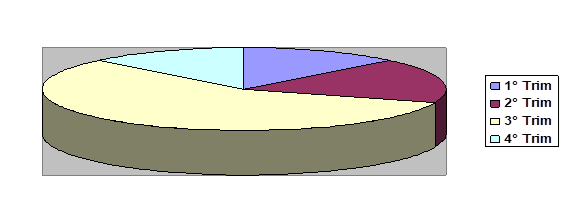
\includegraphics[scale=1.25]{imagens/grafico.png}
	\captionsetup{singlelinecheck=false}
	\legend{\hspace{1cm}\footnotesize\textbf{Fonte: }elaborado pelo autor.}
\end{figure}

As informações que devem ser inseridas nos comandos são apresentadas a seguir.

\subsubsection{Posicionamento da figura no texto}
\label{posiciona}
Nos colchetes ao lado do comando $\backslash$begin\{figure\}[ ] deve ser inserida a informação sobre a posição da figura, da seguinte maneira:

h - para inserir a figura exatamente neste ponto do texto

t - para inserir a figura no topo da página

b - para inserir a figura na base da página



\normalsize
p - para inserir a figura na página\\

Mais de uma opção pode ser utilizada, sendo que a ordem das letras representa a ordem de preferência de posicionamento. Colocar um sinal de exclamação (!) antes das letras significa que o compilador deve forçar o atendimento da configuração definida pelo usuário.

\subsubsection{Título e rótulo da figura}
O título da figura deve ser inserido entre as chaves do comando $\backslash$caption\{ \}. O LaTeX irá numerar a figura automaticamente e apresentar sua numeração e título.

O rótulo da figura é inserido com o comando $\backslash$label\{ \} e serve de identificação para que a figura seja encontrada pelo LaTeX. O rótulo não é mostrado no texto, mas utilizada todas as vezes que queremos chamar a figura ou falar sobre ela. 

\subsubsection{Incluindo a figura}
O comando $\backslash$includegraphics[ ]\{ \} insere a figura no ambiente. Entre os colchetes deve ser informado o dimensionamento da figura. Algumas possibilidades são:

\textbf{width=num} - define a largura da figura. A variável num, após o sinal de igualdade, indica o valor da largura definida para a figura. Deve ser informada a unidade, que pode ser mm, cm, in, pt...

\textbf{height=num} - define a altura da figura.

\textbf{scale=num} - redimensiona a figura na escala definida com base em suas dimensões originais. É possível diminuir (num < 1) ou amentar a figura (num > 1).

\textbf{angle}=num - rotaciona a figura em sentido anti-horário. O argumento \textbf{num} deve informar o ângulo de rotação em graus.

\textbf{width=scale$\backslash$textwidth} - define a largura da figura com relação à largura do texto

\textbf{width=scale$\backslash$paperwidth} - define a largura da figura com relação à largura do papel

\textbf{height=scale$\backslash$paperheight} - define a altura da figura com relação à altura do papel

Entre as chaves deve ser informado o nome do arquivo. Caso a figura esteja em uma subpasta ou em uma pasta diferente dos arquivos .tex, deve-se informar o caminho até a pasta onde está o arquivo  da figura.

\subsubsection{Legenda da figura}
Na legenda, deve-se informar a fonte de onde a figura foi retirada. Caso seja de autoria própria, deve-se escrever ``Elaborado pelo autor''. Caso tenha sido retirada de alguma referência, deve-se fazer a citação dessa referência, utilizando-se o comando $\backslash$cite\{ \}.


\subsubsection{Chamada da figura no texto}
As ilustrações devem ser chamadas no texto, utilizando-se o comando $\backslash$ref\{ \}, inserindo-se o rótulo (label) da figura entre as chaves.

\subsection{Tabelas}
A inserção de tabelas no texto utiliza os ambientes \textit{table} e \textit{tabular}. No primeiro, são definidos elementos como o título, o rótulo e a posição da tabela no texto. Os comandos $\backslash$caption\{ \} e $\backslash$label\{ \}, utilizados com figuras, aplicam-se também a tabelas. As instruções para posicionamento mostradas em \ref{posiciona} também servem para tabelas. No ambiente \textit{tabular} são inseridos os valores que preenchem a tabela, utilizando o símbolo \& como separador de colunas e $\backslash\backslash$ como separador de linhas.

Como as tabelas podem possuir diferentes especificações de linhas e colunas, seguem alguns exemplos:\\

As inclinações recomendadas para os módulos fotovoltaicos para diferentes latitudes são mostradas na Tabela \ref{tab:inclina}.

\begin{table}[h]
\textbf{\caption{Inclinações recomendadas para os módulos fotovoltaicos\label{tab:inclina}}}
\centering
\begin{tabular}{c|c}
\toprule
Latitude geográfica do local & Ângulo de inclinação recomendado \\
\hline
$0^o$ a $10^o$  & $\alpha = 10^o$\\
$0^o$ a $10^o$  & $\alpha = latitude$\\
$0^o$ a $10^o$  & $\alpha = latitude + 5^o$\\
$0^o$ a $10^o$  & $\alpha = latitude + 10^o$\\
acima de $40^o$ & $\alpha = latitude + 15^o$\\
\bottomrule
\end{tabular}
\legend{\footnotesize\textbf{Fonte: }\cite{garcia2020}}
\end{table}

Na Tabela \ref{tab:partes} está esquematizado o padrão recomendado pela NBR 14724 \cite{NBR14724}, que foi elaborado para facilitar a apresentação formal dos trabalhos acadêmicos, na ordem exata em que os elementos devem ser apresentados:

\begin{table}[h]
\bfseries{\caption{Partes que compõem a estrutura do TCC}\label{tab:partes}}
\normalfont
\begin{tabular}{|l|l|l|}
\hline
\multicolumn{2}{|l|}{Parte externa}                                                                     & \begin{tabular}[c]{@{}l@{}}\textbf{Capa}\\\underline{Lombada}\vspace{0.5cm}\end{tabular}                                                                                                                                                                                                                                                                                                                                                                         \\ \hline
\multirow{3}{*}{Parte interna} & \begin{tabular}[c]{@{}l@{}}Elementos\\pré-textuais\end{tabular} & \begin{tabular}[c]{@{}l@{}}\textbf{Folha de rosto}\\\textbf{Ficha catalográfica (no verso da folha de rosto)}\\\underline{Errata}\\\textbf{Folha de aprovação}\\\underline{Dedicatória}\\  \underline{Agradecimentos}\\\underline{Epígrafe}\\\textbf{Resumo na língua vernácula}\\\textbf{Resumo em língua estrangeira}\\\underline{Lista de ilustrações}\\\underline{Lista de tabelas}\\\underline{Lista de abreviaturas e siglas}\\\underline{Lista de símbolos}\\\textbf{Sumário}\end{tabular} \\ \cline{2-3} 
                               & \begin{tabular}[c]{@{}l@{}}Elementos\\textuais\end{tabular}     & \begin{tabular}[c]{@{}l@{}}\textbf{Introdução}\\\textbf{Desenvolvimento}\\\textbf{Conclusão}\end{tabular}                                                                                                                                                                                                                                                                                                                                         \\ \cline{2-3} 
                               & \begin{tabular}[c]{@{}l@{}}Elementos\\pós-textuais\end{tabular} & \begin{tabular}[c]{@{}l@{}}\textbf{Referências}\\\underline{Glossário}\\\underline{Apêndice(s)}\\\underline{Anexo(s)}\\\underline{Índice}\end{tabular}                                                                                                                                                                                                                                                                                                            \\ \hline
\multicolumn{3}{|l|}{\begin{tabular}[c]{@{}l@{}}\textbf{Elementos obrigatórios}\\\underline{Elementos opcionais}\end{tabular}}                                                                                                                                                                                                                                                                                                                                                                                                                               \\ \hline
\end{tabular}
\legend{\footnotesize\textbf{Fonte:} adaptada de \cite{NBR14724}} %Indicar a autoria da Tabela
\end{table}

\textbf{Nota: }para inserir tabelas no texto é possível utilizar os assistentes do TexMaker. A explicação de como utilizá-los está na série de vídeo-aulas.


\section{Expressões Matemáticas}
Expressões matemáticas, como fórmulas, sistemas de equações, matrizes, etc., podem ser inseridas na mesma linha do texto ou à parte dele, dando maior destaque à expressão. Nesta seção serão mostradas algumas formas de se construir essas expressões no texto.

\subsection{Fórmulas na mesma linha do texto}
Para inserir uma fórmula simples na mesma linha do texto, basta escrever a expressão entre \$\$. Exemplo:

Para um triângulo retângulo, pode-se escrever que $a^2+b^2=c^2$, sendo $a$ e $b$ os catetos e $c$ a hipotenusa do triângulo.


\subsection{Fórmulas destacadas do texto}
As expressões matemáticas podem ser destacadas do texto para facilitar a leitura. Se necessário pode-se numerá-las com algarismos arábicos entre parênteses alinhados à direita, como (\ref{eq1}) e (\ref{eq2}). Para as fórmulas é permitida uma entrelinha maior para comportar os expoentes e índices. Para destacar as expressões do texto, utiliza-se o ambiente \textbf{equation}. Para chamar as expressões no texto, é necessário nelas colocar um rótulo, utilizando o comando $\backslash$label\{ \} logo após iniciar o ambiente equation.

Exemplos:\\

\noindent
$\backslash$begin\{equation\}\\
$\backslash$label\{eq1\}\\
x\string^2+x\string^3=n\\
$\backslash$end\{equation\}\\

retorna:

\begin{equation}
\label{eq1}
x^2+x^3=n
\end{equation}

Já o código:\\

\noindent
$\backslash$begin\{equation\}\\
$\backslash$label\{eq2\}\\
x=$\backslash$frac\{-b $\backslash$pm $\backslash$sqrt\{$\backslash$Delta\}\}\{2.a\}\\
$\backslash$end\{equation\}

retorna:

\begin{equation}
\label{eq2}
x=\frac{-b \pm \sqrt{\Delta}}{2.a}
\end{equation}

Os caracteres especiais, como símbolos matemáticos e letras gregas são inseridos por comandos, como $\backslash$pm, que insere o sinal de mais/menos ou $\backslash$Delta, que insere a letra grega $\Delta$. Contudo, é possível utilizar os assistentes do Texmaker para inserir esses símbolos sem que seja necessário memorizar todos os comandos.

Caso a expressão não precise ser numerada, utilize o ambiente \textbf{$\backslash$equation*}. Exemplo:\\

\noindent
$\backslash$begin\{equation*\}\\
$\backslash$label\{eq3\}\\
V\_\{Lmed\} = 0,225 $\backslash$times (1-cos$\backslash$beta)\\
$\backslash$end\{equation*\}\\

retorna:

\begin{equation*}
\label{eq3}
V_{Lmed} = 0,225 \times (1-cos\beta)
\end{equation*}

\subsection{Expressões longas}
Caso a expressão a ser apresentada seja muito longa, é possível quebrá-la e inseri-la em mais de uma linha utilizando o ambiente \textbf{multiline}. A quebra da equação não é automática e deve ser definida pelo usuário.\\

\noindent
$\backslash$begin\{multline\}\\
p(x) = 3x\string^6 + 14x\string^5y + 590x\string^4y\string^2 + 19x\string^3y\string^3 - 10x\string^3y\string^2 + 6x\string^2y\string^5 + 33x\string^2y\string^4$\backslash\backslash$\\ 
- 12x\string^2y\string^3 - 12xy\string^5 + 2y\string^6 - a\string^3b\string^3\\
$\backslash$end\{multline\}\\

retorna:\\
\begin{multline}
p(x) = 3x^6 + 14x^5y + 590x^4y^2 + 19x^3y^3 - 10x^3y^2 + 6x^2y^5 + 33x^2y^4\\ 
- 12x^2y^3 - 12xy^5 + 2y^6 - a^3b^3\\
\end{multline}

\subsection{Conjuntos de expressões}
Quando for necessário alinhar várias equações, pode-se utilizar o ambiente \textbf{align}. O símbolo $\&$ indica o ponto de alinhamento entre as equações. Assim, o código:\\

\noindent
$\backslash$begin\{align\}\\
3x + 2y + 5z $\&$ = 10$\backslash\backslash$\\
2x - y + 3z $\&$ = 4$\backslash\backslash$\\
2y + z $\&$ = 6
$\backslash$end\{align\} \\

Retorna as expressões alinhadas no sinal de igualdade:

\begin{align}
3x + 2y + 5z &= 10\\
2x - y + 3z &= 4\\
2y + z &= 6 
\end{align}

Outra opção é a utilização do ambiente \textbf{$\backslash$array}, que pode ser utilizado para alinhar expressões ou para construir matrizes ou outras estruturas em que exista a necessidade de alinhamento. A principal vantagem seste ambiente em comparação com o ambiente $\backslash$align é que ele permite o alinhamento de vários pontos na expressão, utilizando o símbolo \&. Além disso, ele permite determinar se o alinhamento será à esquerda (\textbf{l}eft), centralizado (\textbf{c}enter) ou à direita (\textbf{r}ight). Porém, ele deve ser inserido em um ambiente matemático, por exemplo, o ambiente equation. Exemplos:

O mesmo sistema de equações anterior pode ter todos os seus termos alinhados utilizando o código a seguir.\\

\noindent
$\backslash$begin\{equation\}\\
$\backslash$begin\{array\}\{rrrlr\}\\
3x \&+ 2y \&+ 5z \&= \&10$\backslash\backslash$\\
2x \&- y \&+ 3z \&= \&4$\backslash\backslash$\\
\&2y \&+ z \&= \&6 \\
$\backslash$end\{array\}\\
$\backslash$end\{equation\}

Tem-se, então a saída a seguir. Observe que os termos das equações estão alinhados à direita, mantendo o alinhamento nas variáveis.

\begin{equation}
\begin{array}{rrrlr}
3x &+ 2y &+ 5z &= &10\\
2x &- y &+ 3z &= &4\\
&2y &+ z &= &6 
\end{array}
\end{equation}

O valor de uma função para diferentes condições pode ser mostrado, por exemplo:\\

\noindent
$\backslash$begin\{equation\}\\
|x| = $\backslash$left$\backslash$\{ $\backslash$begin\{array\}\{ll\}\\
         x \& $\backslash$mbox\{if \$x $\backslash$geq 0\$\};$\backslash\backslash$\\
        -x \& $\backslash$mbox\{if \$x < 0\$\}.\\
        $\backslash$end\{array\} $\backslash$right.\\
$\backslash$end\{equation\}\\

retorna: 

\begin{equation}
|x| = \left\{ \begin{array}{ll}
         x & \mbox{if $x \geq 0$};\\
        -x & \mbox{if $x < 0$}.
        \end{array} \right. 
\end{equation}

Agora, um exemplo de montagem de uma matriz. O código a seguir retorna a matriz \ref{matriz}.\\

\noindent
$\backslash$begin\{equation\}\\
$\backslash$left[ $\backslash$begin\{array\}\{ccc\}\\
a \& b \& c $\backslash\backslash$\\
d \& e \& f $\backslash\backslash$\\
g \& h \& i $\backslash$end\{array\} $\backslash$right]\\
$\backslash$end\{equation\}

\begin{equation}
\label{matriz}
\left[ \begin{array}{ccc}
a & b & c \\
d & e & f \\
g & h & i \end{array} \right]
\end{equation}


\chapter{INTRODUÇÃO}

A avaliação de risco de crédito é um dos pilares fundamentais do setor bancário, determinando a viabilidade de concessão de empréstimos e mitigando possíveis inadimplências \cite{khandani2010consumer}. Com o avanço das tecnologias de Inteligência Artificial (IA), especificamente os Grandes Modelos de Linguagem (LLMs) e o Processamento de Linguagem Natural (NLP), surgem novas oportunidades para automatizar e aprimorar processos de análise complexos \cite{araci2019finbert}.

No entanto, instituições financeiras enfrentam grandes desafios ao adotar IA baseada em nuvem devido a regulações rigorosas de privacidade de dados, como a Lei Geral de Proteção de Dados (LGPD) no Brasil e a \textit{General Data Protection Regulation} (GDPR) na Europa. O envio de dados financeiros sensíveis para APIs proprietárias externas compromete o sigilo bancário.

Neste contexto, apresenta-se o projeto CreditMaster, um microsserviço de Inteligência Artificial Generativa (\textit{headless}) projetado especificamente para o setor bancário. Seu principal objetivo é automatizar o fluxo de análise de risco e gerar pareceres técnicos de crédito de forma automática, operando de maneira 100\% \textit{on-premise} (local).

\section{Objetivos}

O objetivo principal deste trabalho é descrever o desenvolvimento e a implementação do CreditMaster como uma ferramenta segura e eficiente de apoio à decisão no processo de análise de crédito.

Os objetivos específicos incluem:
\begin{itemize}
    \item Desenvolver uma arquitetura baseada em LLMs capaz de rodar localmente, garantindo o sigilo bancário e a conformidade com as leis de proteção de dados.
    \item Implementar técnicas de \textit{Fine-Tuning} para internalizar o jargão técnico bancário e padronizar o formato dos pareceres de crédito.
    \item Integrar a técnica de \textit{Retrieval-Augmented Generation} (RAG) para consulta de manuais de crédito e normativas em tempo real, reduzindo alucinações matemáticas e regulatórias.
    \item \textbf{[ANOTAÇÃO: Lembrar de colocar aqui outros objetivos específicos sobre como validei o modelo e as métricas de desempenho que usei.]}
\end{itemize}

\section{Justificativa}

Sob a perspectiva de negócios, a automação da análise de crédito representa um imenso potencial de redução de custos operacionais e agilidade na liberação de limites para os clientes. Processos tradicionais dependem de longas revisões humanas em bases de dados e manuais extensos. A utilização de Inteligência Artificial para gerar o parecer técnico primário libera os analistas humanos para atuarem apenas na aprovação final e no tratamento de exceções, conferindo alta escalabilidade às instituições financeiras.

Sob a ótica tecnológica, até recentemente, a implementação de IA generativa no ambiente corporativo estava restrita a serviços de nuvem controlados por \textit{Big Techs}, gerando impasses jurídicos de privacidade e compliance (como a LGPD e regulamentações do BACEN). A maturação de Modelos de Linguagem de código aberto e tamanho otimizado (como o Llama 3.1 com 8 bilhões de parâmetros), combinada a técnicas de quantização (QLoRA), tornou viável rodar inferências sofisticadas localmente em hardwares de baixo custo (e.g., placas de vídeo de consumo geral como a RTX 5060 Ti). Portanto, o desenvolvimento deste trabalho justifica-se por demonstrar a plena factibilidade técnica e econômica de aplicar IA de ponta respeitando restrições rígidas de sigilo bancário.

\chapter{FUNDAMENTAÇÃO TEÓRICA}

Este capítulo aborda os conceitos fundamentais que baseiam a arquitetura do CreditMaster, focando no uso de Modelos de Linguagem e técnicas avançadas de engenharia de \textit{prompt} e adaptação de modelos.

\section{Modelos de Linguagem de Grande Escala (LLMs)}

A área de Processamento de Linguagem Natural (NLP) sofreu uma transformação radical com o advento de arquiteturas baseadas em redes neurais profundas (\textit{Deep Learning}). Conforme delineado por \citeonline{lecun2015deeplearning}, o aprendizado profundo permite que modelos computacionais compostos por múltiplas camadas de processamento aprendam representações de dados com múltiplos níveis de abstração. Na seara do NLP, essa evolução culminou na arquitetura \textit{Transformer}, introduzida por \citeonline{vaswani2017attention}, que dispensou os componentes recorrentes e convolucionais baseando-se inteiramente em mecanismos de "atenção". Esse marco permitiu paralelização massiva e o treinamento de Modelos de Linguagem de Grande Escala (LLMs) com bilhões, e eventualmente trilhões, de parâmetros.

Os LLMs são sistemas treinados em vastos \textit{corpora} de texto da internet com o objetivo de prever o próximo \textit{token} (palavra ou sub-palavra) em uma sequência, o que lhes confere notável habilidade de gerar textos coerentes e contextuais. No escopo deste projeto, o modelo \textbf{Llama 3.1 8B Instruct}, desenvolvido de forma \textit{open-source} pela Meta, destaca-se por oferecer uma relação custo-benefício excepcional. Com 8 bilhões de parâmetros, ele atinge um equilíbrio ideal, sendo poderoso o suficiente para assimilar o intrincado jargão financeiro, mas compacto o bastante para ser executado integralmente \textit{on-premise} (localmente) em uma única GPU, evitando gargalos e riscos inerentes ao envio de dados sigilosos para a nuvem.

\section{\textit{Fine-Tuning} e QLoRA}
O ajuste fino (\textit{Fine-Tuning}) completo de modelos com bilhões de parâmetros exige altíssimo poder computacional. Para contornar esse desafio técnico, utiliza-se o método QLoRA (\textit{Quantized Low-Rank Adaptation}), que permite modificar estruturalmente os pesos neurais do modelo base com uso otimizado e drástico de memória. No projeto, a biblioteca \textbf{Unsloth} é utilizada para acelerar esse processo e viabilizar o treinamento em GPUs convencionais.

\section{\textit{Retrieval-Augmented Generation} (RAG)}
A Geração Aumentada por Recuperação (RAG) consiste na injeção dinâmica de contexto factual no momento da inferência do modelo. Para o domínio bancário, a eliminação de "alucinações" (geração de textos plausíveis, porém incorretos ou inventados) é um requisito crítico. A arquitetura RAG permite consultas contra manuais internos e políticas de crédito, garantindo que o modelo responda estritamente de acordo com as regras estabelecidas, mantendo a rastreabilidade do processo decisório.
\textbf{[ANOTAÇÃO: Tenho que expandir essa explicação sobre os bancos vetoriais, falando mais do ChromaDB e FAISS que usei pra salvar e buscar os documentos.]}

\chapter{METODOLOGIA E DESENVOLVIMENTO}

O CreditMaster foi idealizado sob uma arquitetura híbrida focada em segurança, eficiência e precisão para o setor financeiro. O diferencial técnico reside no fato da operação de maneira autônoma e 100\% local (\textit{on-premise}), assegurando a proteção de dados sigilosos e o cumprimento de marcos legais como LGPD, mitigando a dependência de APIs em nuvem.

\section{Arquitetura Híbrida do Sistema}
O núcleo de tomada de decisão do sistema opera através da composição sinérgica de duas técnicas de IA generativa:

\subsection{Ajuste Fino (QLoRA) com Llama 3.1 8B}
O modelo base selecionado foi o \textbf{Llama 3.1 8B Instruct}. A modificação estrutural de seus parâmetros foi viabilizada pela utilização da biblioteca \textbf{Unsloth}, e o modelo final foi exportado no formato \textbf{GGUF} para execução local otimizada. 
Esta etapa atingiu os seguintes propósitos:
\begin{itemize}
    \item Internalização de jargões técnicos do meio bancário e financeiro.
    \item Padronização rigorosa do formato sintático dos pareceres de análise de crédito.
    \item Otimização extrema no uso de memória para permitir inferências ultrarrápidas em \textit{hardware} local, especificamente utilizando o ecossistema CUDA Toolkit em GPUs NVIDIA.
\end{itemize}

\subsection{Motor RAG (\textit{Retrieval-Augmented Generation})}
\textbf{[ANOTAÇÃO: RAG não foi implementado ainda.]}

\section{Construção do Conjunto de Dados (\textit{Dataset})}
A qualidade do modelo \textit{fine-tuned} depende diretamente da qualidade dos dados. O repositório do CreditMaster estrutura-se sobre dados proprietários contendo:
\begin{itemize}
    \item \textbf{Políticas de Crédito:} Documentos que definem diretrizes de concessão e risco de mercado (\texttt{credit\_policy\_pt.md}). \textbf{[ANOTAÇÃO: A politica vai ser implementada ao modelo junto com o RAG.]}
    \item \textbf{Histórico de Pareceres:} Uma base sintética contendo milhares de exemplos rotulados (\texttt{pareceres\_credito\_2000.jsonl}), construída através de metodologias automatizadas de roteirização (\texttt{gerar\_pareceres.py}). \textbf{[ANOTAÇÃO: Como não tive acesso a pareceres reais, utilizei uma base de dados da Lending Club disponibilizadas via Kaggle e gerei pareceres sintéticos.]}
\end{itemize}
A base de dados foi construída com base em 14 variáveis centrais: valor do empréstimo (\texttt{loan\_amnt}), prazo (\texttt{term}), tempo de emprego (\texttt{emp\_length}), tipo de moradia (\texttt{home\_ownership}), renda anual (\texttt{annual\_inc}), finalidade (\texttt{purpose}), relação dívida/renda (\texttt{dti}), pontuação mínima de crédito (\texttt{fico\_range\_low}), atrasos nos últimos 2 anos (\texttt{delinq\_2yrs}), consultas nos últimos 6 meses (\texttt{inq\_last\_6mths}), utilização do limite rotativo (\texttt{revol\_util}), número de contas ativas abertas (\texttt{open\_acc}), ocorrência de registros públicos (\texttt{pub\_rec}) e o status histórico do contrato (\texttt{loan\_status}).

Os dados foram convertidos por meio de rotinas em Python (\texttt{gerar\_pareceres.py}) para o formato padrão de conversação \textit{Chat Template} do Llama 3.1 no formato JSONL (\texttt{pareceres\_credito\_2000.jsonl}), contendo as mensagens de sistema (\textit{system prompt}), a requisição estruturada do usuário com as métricas financeiras do cliente e a conclusão técnica gerada em formato JSON (\textit{assistant}). Do total de 1.998 amostras processadas, 1.698 (85\%) foram alocadas para o conjunto de treinamento e 300 (15\%) para o conjunto de validação e teste.

\section{Visão Geral das Tecnologias Aplicadas}
Para suportar o rigor da arquitetura, o \textit{Tech Stack} consolidou as seguintes soluções:
\begin{itemize}
    \item \textbf{Camada de IA e Modelagem:} Python 3.10+, Llama 3.1 8B, Unsloth, QLoRA e exportação GGUF.
    \item \textbf{Motor de Inferência:} Ambiente Linux Mint suportando Ollama e CUDA Toolkit.
    \item \textbf{Pipeline de Dados:} Pandas. \textbf{[ANOTAÇÃO: Aqui serão também, adicionados o utilizado para o RAG]}
\end{itemize}
 
\chapter{RESULTADOS E DISCUSSÕES}

Neste capítulo são apresentados e discutidos os resultados experimentais obtidos durante o processo de treinamento, quantização e inferência do \textit{CreditMaster}. A avaliação abrange tanto o desempenho computacional da arquitetura QLoRA executada em \textit{hardware} local de consumo quanto a análise da dinâmica de convergência da perda (\textit{loss}), o comportamento da taxa de aprendizado (\textit{learning rate schedule}) e a qualidade semântica dos pareceres técnicos de crédito gerados.

\section{Ambiente Computacional e Eficiência de Recursos}

O treinamento supervisionado (\textit{Supervised Fine-Tuning} - SFT) foi conduzido inteiramente em ambiente local (\textit{on-premise}), validando a hipótese de viabilidade de modelos de 8 bilhões de parâmetros em infraestruturas acessíveis ao setor corporativo. A estação de trabalho utilizada contou com a seguinte configuração de \textit{hardware} e \textit{software}:
\begin{itemize}
    \item \textbf{Processador (CPU):} AMD Ryzen 5 7600X (6 núcleos físicos, 12 \textit{threads}, clock base de 4.7 GHz);
    \item \textbf{Memória Principal (RAM):} 16 GB DDR5 com frequência de 6000 MHz;
    \item \textbf{Armazenamento Secundário:} Unidade de Estado Sólido (SSD) NVMe PCIe 3.0;
    \item \textbf{Unidade de Processamento Gráfico (GPU):} NVIDIA GeForce RTX 5060 Ti com 8 GB de VRAM física (7,52 GB utilizáveis);
    \item \textbf{Sistema Operacional e Frameworks:} Linux Mint 22 (base Ubuntu 24.04 LTS), PyTorch 2.10.0+cu128, CUDA Toolkit 12.8, HuggingFace TRL 0.24.0, Transformers 5.5.0 e biblioteca Unsloth.
\end{itemize}

A aplicação da técnica QLoRA associada à quantização NF4 (\textit{4-bit NormalFloat}) e à biblioteca Unsloth permitiu uma redução drástica na pegada de memória de vídeo. Durante todo o ciclo de 2 épocas (426 passos de otimização), o pico de alocação de VRAM registrado foi de \textbf{6,44 GB}, representando uma ocupação média de aproximadamente 85,7\% da capacidade total da GPU. Esse comportamento comprova que a técnica evita falhas por estouro de memória (\textit{Out of Memory} - OOM). Além disso, a utilização da memória RAM convencional do sistema manteve-se baixa (inferior a 2,5 GB alocados ao processo de treino), visto que as operações matriciais massivas e o armazenamento de gradientes foram concentrados diretamente nos núcleos tensores da GPU.

A Tabela~\ref{tab:metricas_treinamento} consolida os parâmetros de treinamento e as métricas computacionais globais obtidas.

\begin{table}[htbp]
\centering
\caption{Métricas e Resultados Computacionais do Ajuste Fino (QLoRA)}
\label{tab:metricas_treinamento}
\begin{tabular}{ll}
\hline
\textbf{Parâmetro / Métrica} & \textbf{Valor Obtido} \\ \hline
Modelo Base & Meta Llama 3.1 8B Instruct (4-bit NF4) \\
Hardware Utilizado & NVIDIA GeForce RTX 5060 Ti (8 GB VRAM) \\
Amostras de Treino (85\%) & 1698 \\
Amostras de Validação (15\%) & 300 \\
Tamanho Efetivo do Batch & 8 (Batch 2 $\times$ Acumulação de Gradientes 4) \\
Épocas de Treinamento & 2,0 \\
Total de Passos de Otimização & 426 \\
Perda Inicial de Treino ($L_{inicial}$) & 1,3272 \\
Perda Final de Treino ($L_{train}$) & 0,0046 \\
Perda Final de Validação ($L_{val}$) & 0,0045 \\
Taxa de Redução da Perda & 99,65\% \\
Tempo Total de Ajuste Fino & 75,63 minutos (4.537,99 segundos) \\
Vazão de Treinamento (\textit{Throughput}) & 0,748 amostras/s \\
Pico de Alocação de VRAM & 6,44 GB / 7,52 GB (85,7\%) \\ \hline
\end{tabular}
\fonte{Elaborado pelo autor (2026).}
\end{table}

\section{Dinâmica de Treinamento e Convergência da Perda}

O aprendizado e a capacidade de generalização do modelo foram avaliados a partir da evolução da função de perda por entropia cruzada (\textit{Cross-Entropy Loss}) ao longo das iterações de treino e validação. A Figura~\ref{fig:curva_perda} apresenta as curvas de $L_{train}$ e $L_{val}$ coletadas a cada intervalo de avaliação.

\begin{figure}[H]
    \centering
    \caption{Curva de convergência de perda de treinamento e validação no ajuste fino QLoRA.}
    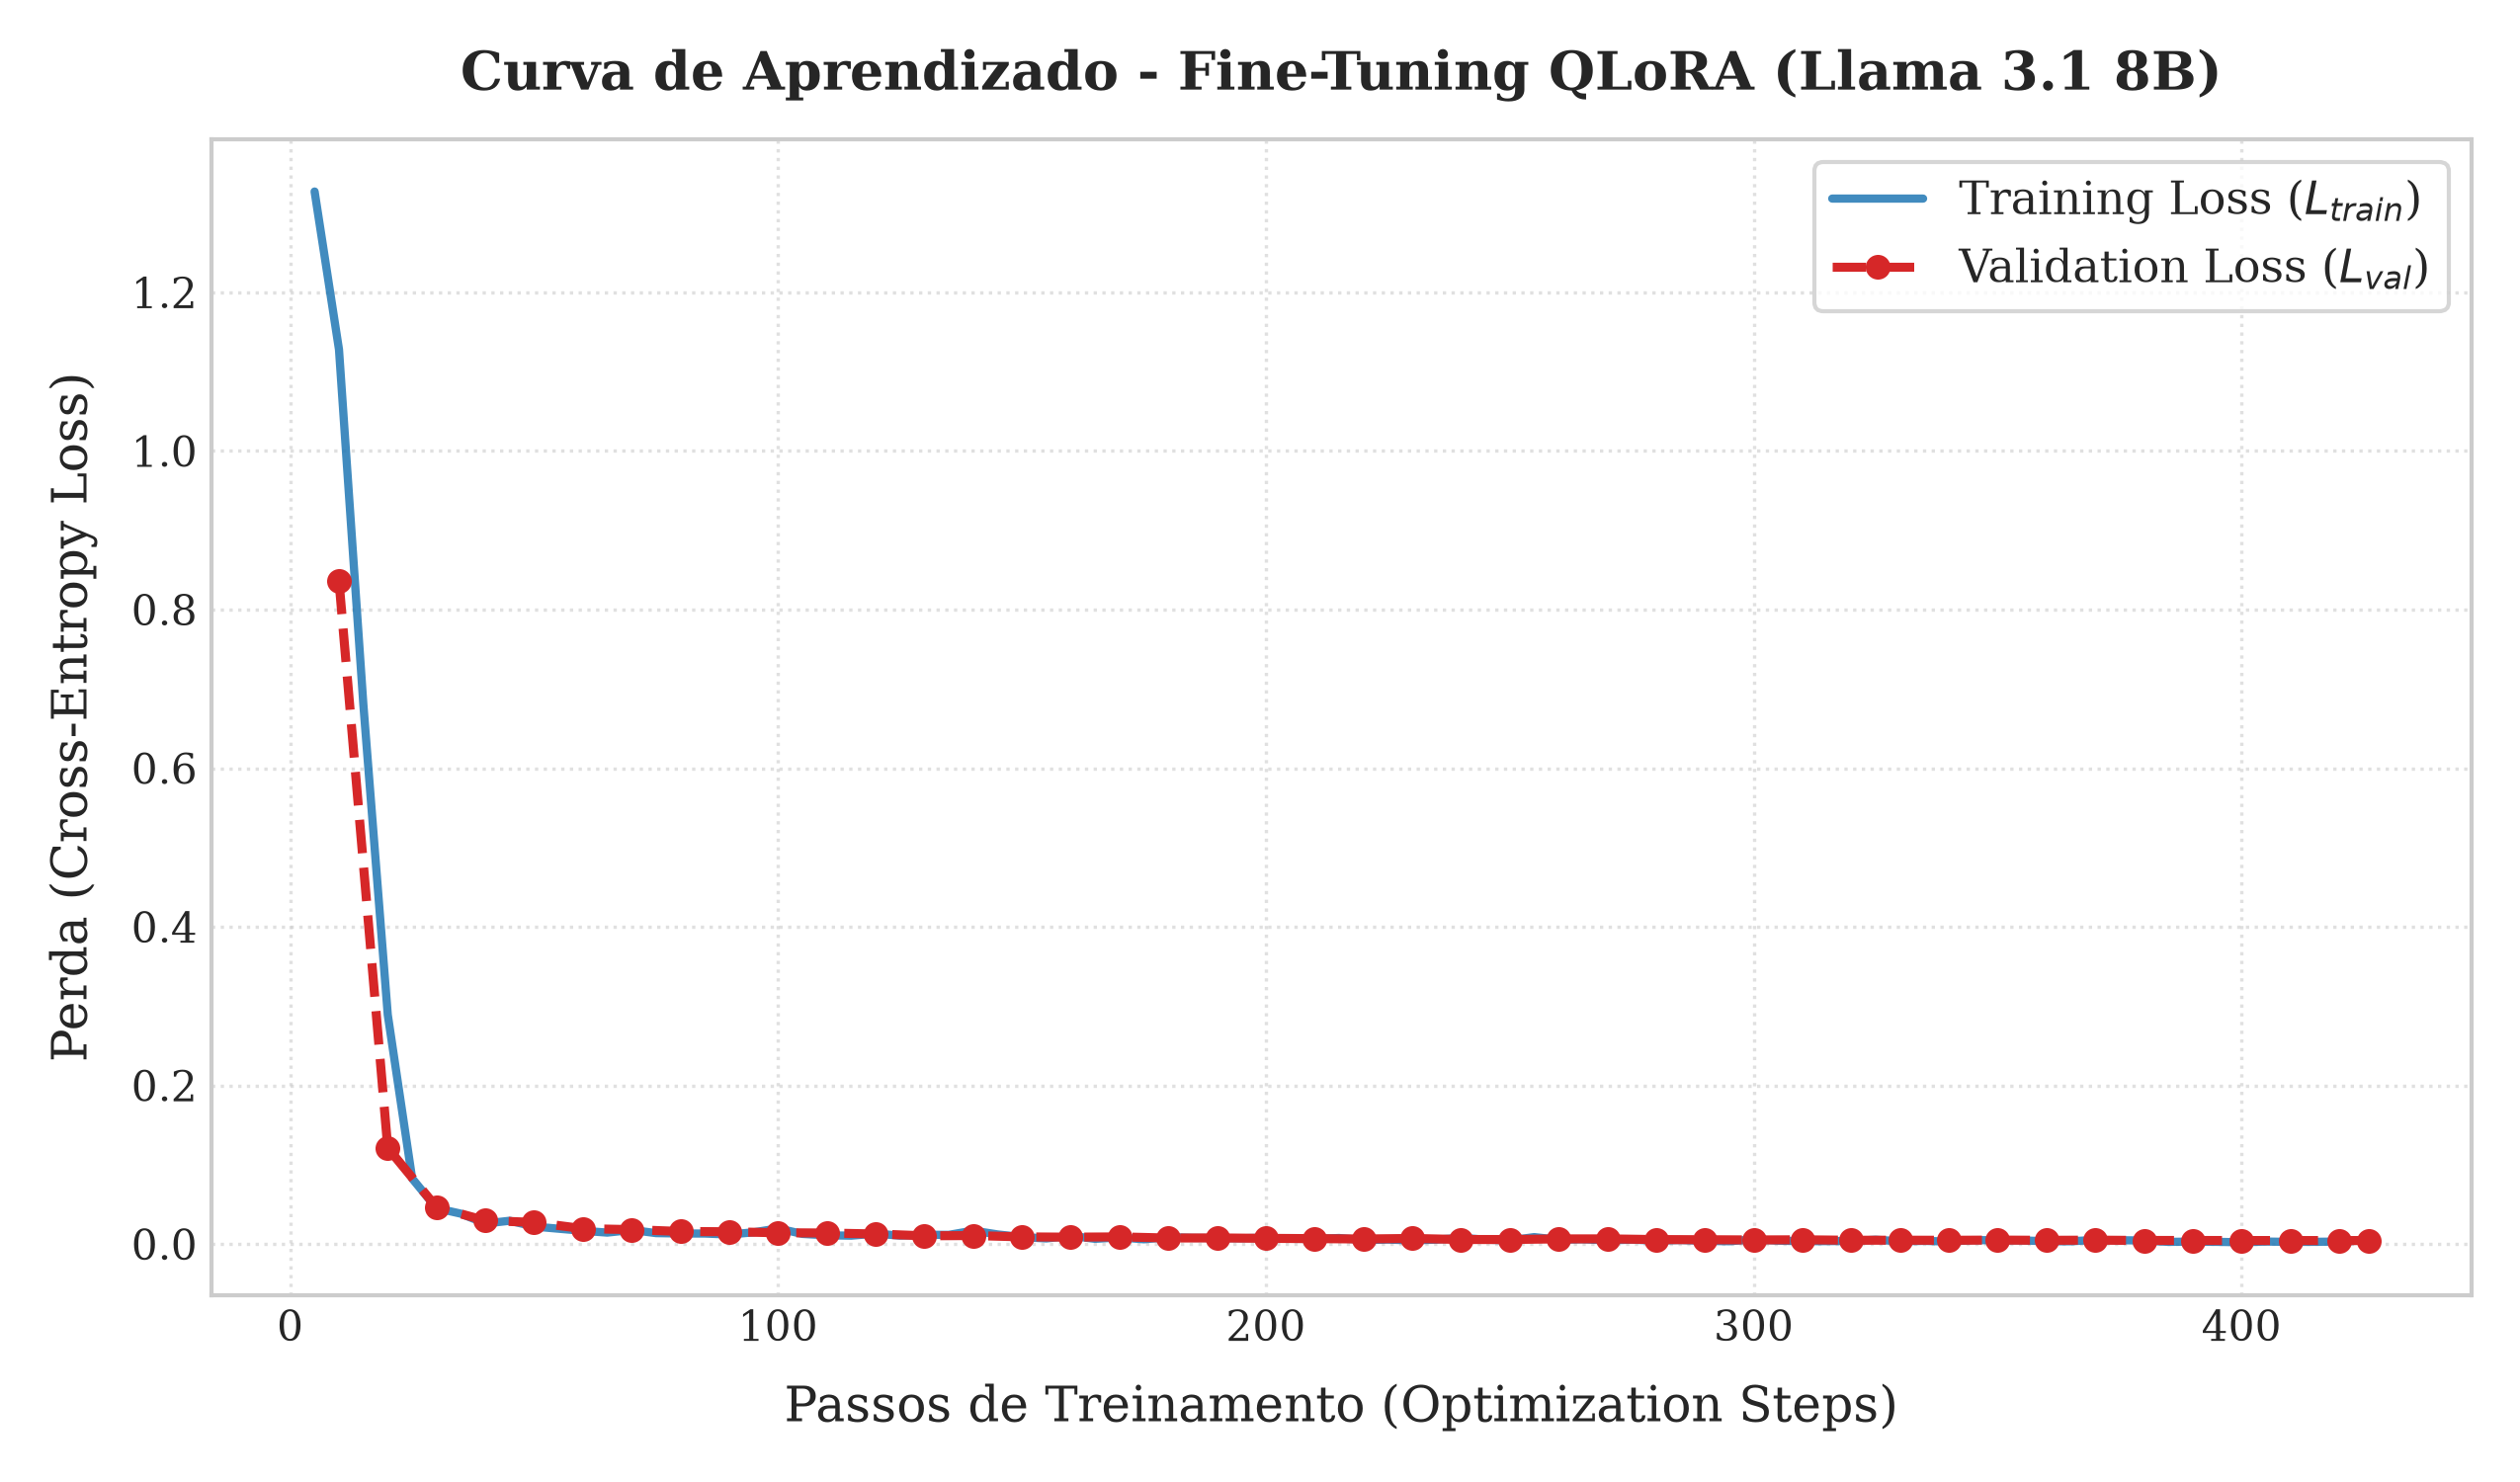
\includegraphics[width=0.92\textwidth]{imagens/curva_perda_treinamento.png}
    \fonte{Elaborado pelo autor (2026).}
    \label{fig:curva_perda}
\end{figure}

A análise detalhada da trajetória de perda revela três períodos distintos:

\begin{enumerate}
    \item \textbf{Fase de Adaptação Sintática Inicial (Passos 1 a 40 / 0,0 a 0,2 épocas):} Nos primeiros passos, observa-se uma queda exponencial na perda de treino, de $1,3272$ no passo 5 para $0,0260$ no passo 40, enquanto a perda de validação foi reduzida de $0,8364$ (passo 10) para $0,0297$ (passo 40). Esse comportamento está relacionado à rápida adaptação dos parâmetros LoRA à estrutura de saída em JSON estrito, o delimitador de instrução do \textit{Llama 3.1 Chat Template} e a técnica de mascaramento \texttt{train\_on\_responses\_only}, na qual a perda é computada exclusivamente sobre os \textit{tokens} gerados pelo assistente.
    
    \item \textbf{Fase de Refinamento Semântico e Regras de Negócio (Passos 40 a 200 / 0,2 a 0,94 épocas):} O modelo apresenta uma redução gradual da função de perda, com $L_{train}$ passando de $0,0260$ para $0,0082$ e $L_{val}$ atingindo $0,0073$. Nessa etapa, os adaptadores neurais ajustam os parâmetros do modelo para representar as relações não lineares entre as variáveis financeiras, como DTI, faixa de FICO, número de atrasos e recomendação de crédito.
    
    \item \textbf{Fase de Convergência Assintótica e Minimização de Ruído (Passos 200 a 426 / 0,94 a 2,0 épocas):} A perda é estabilizada em milésimos, finalizando em $L_{train} = 0,0046$ e $L_{val} = 0,0045$. A proximidade estrita entre as curvas de validação e treinamento ($L_{val} \approx L_{train}$) durante todo o processo comprova matematicamente a \textbf{ausência de sobreajuste (\textit{overfitting})}, demonstrando que o modelo generalizou os conceitos sem memorizar cegamente as amostras de treinamento.
\end{enumerate}

\section{Evolução do Agendamento da Taxa de Aprendizado}

Para assegurar estabilidade numérica no espaço de parâmetros de baixa dimensionalidade do LoRA ($r=16, \alpha=16$), utilizou-se um agendador com aquecimento linear (\textit{Linear Warmup}) seguido por decaimento cosseno (\textit{Cosine Decay Schedule}). A Figura~\ref{fig:taxa_aprendizado} ilustra a evolução da taxa de aprendizado ao longo dos 426 passos.

\begin{figure}[H]
    \centering
    \caption{Agendamento da Taxa de Aprendizado (\textit{Cosine Decay with Warmup}).}
    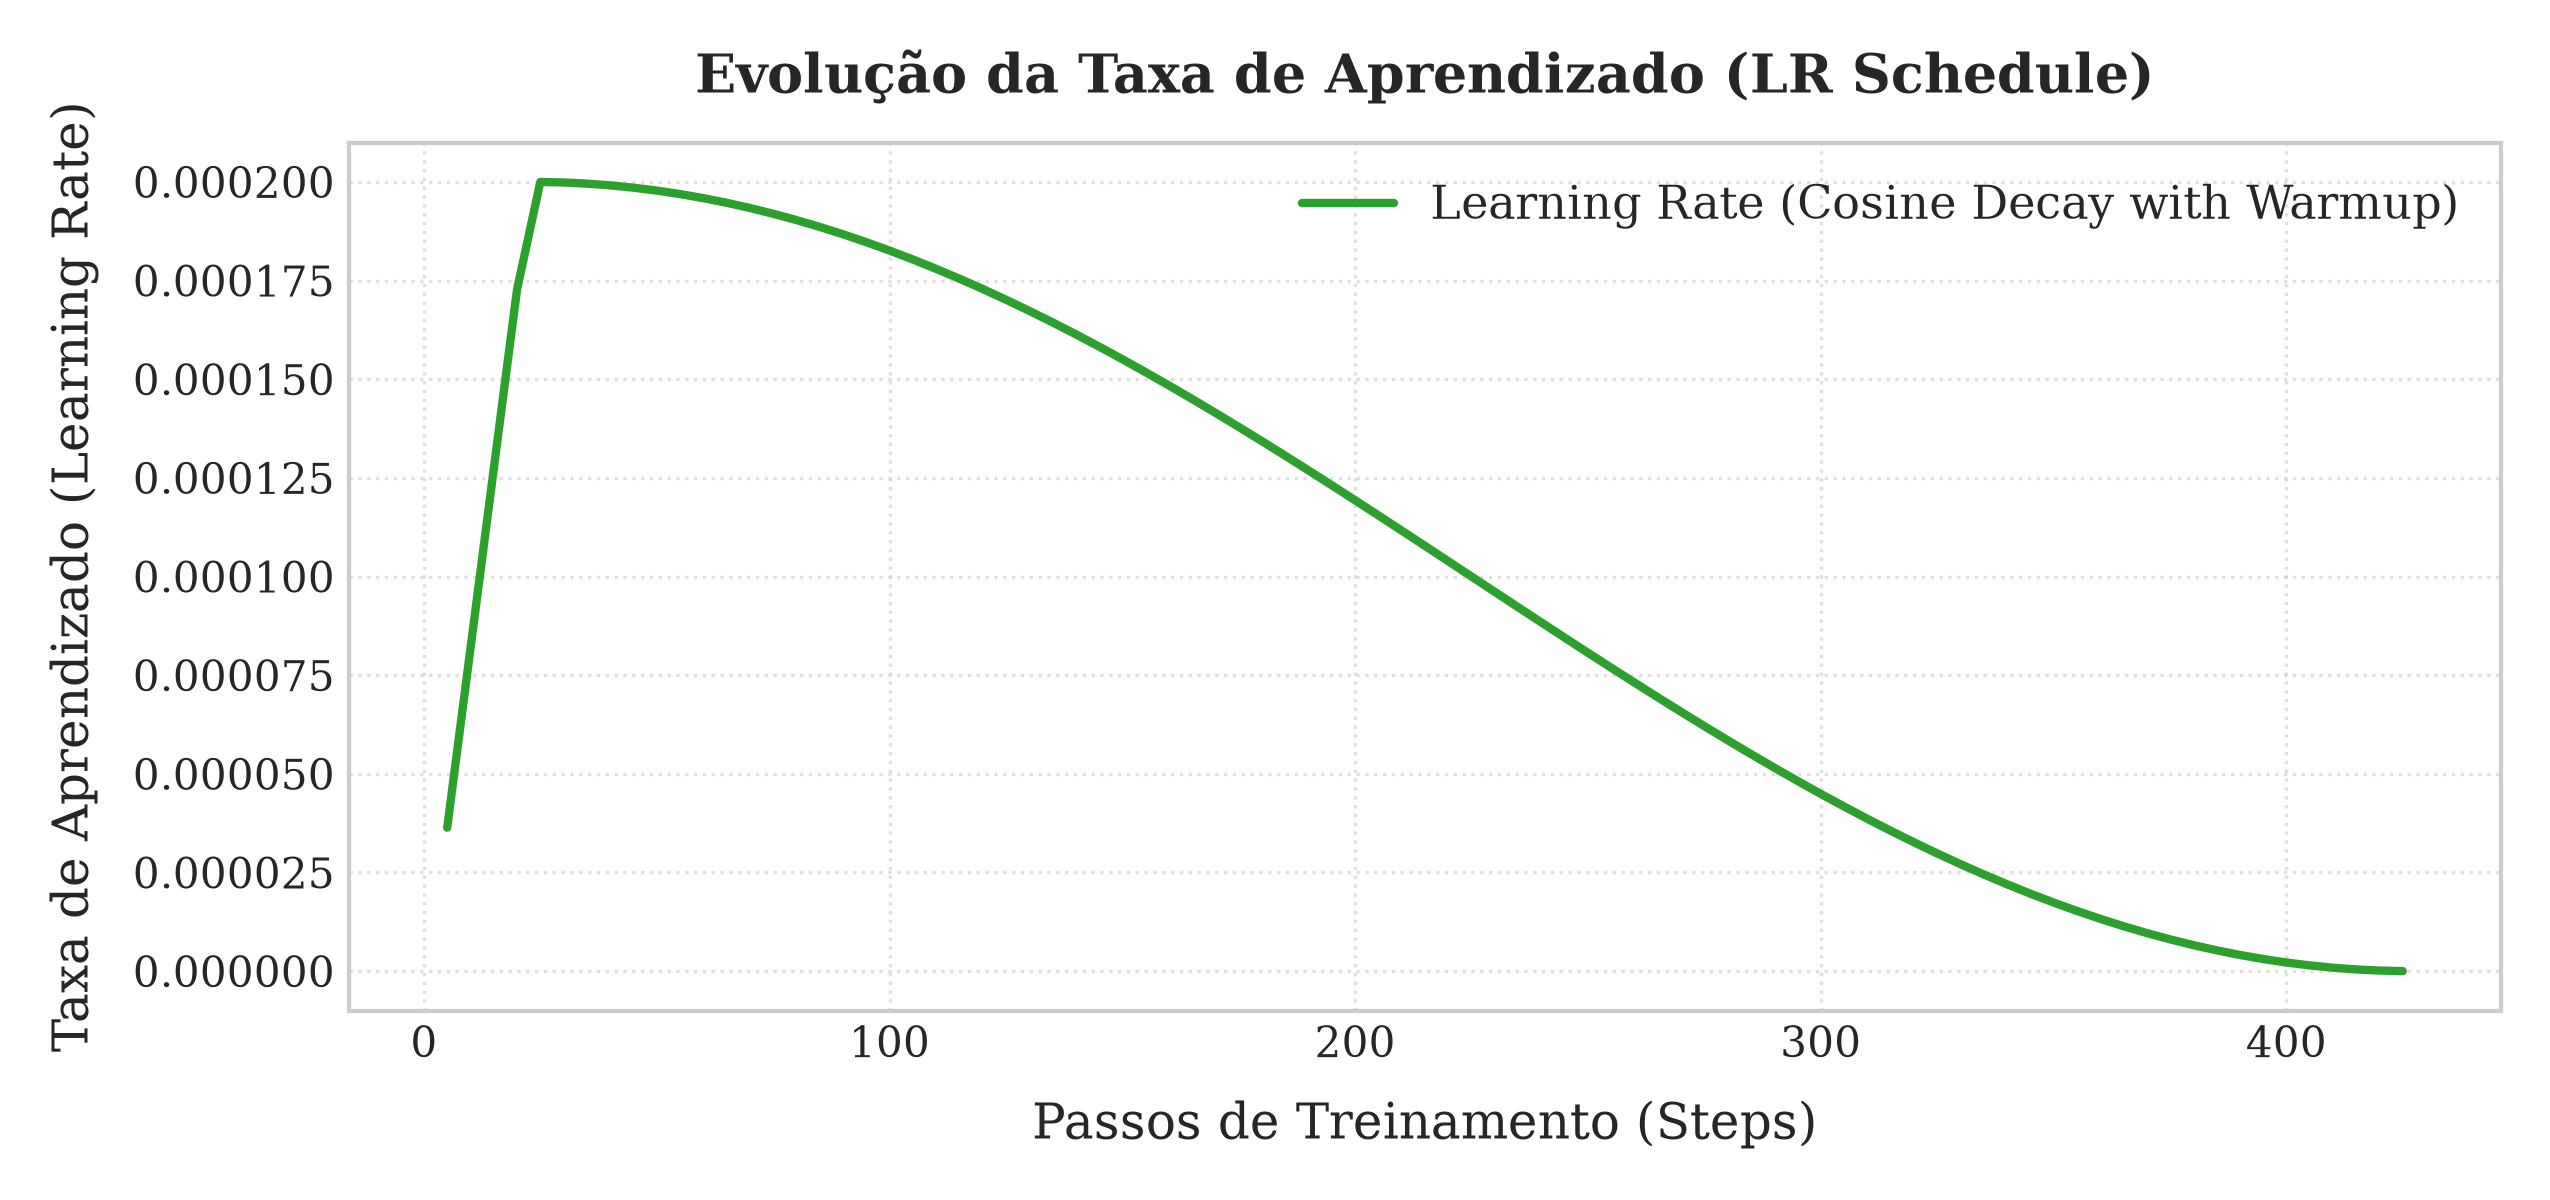
\includegraphics[width=0.92\textwidth]{imagens/taxa_aprendizado.png}
    \fonte{Elaborado pelo autor (2026).}
    \label{fig:taxa_aprendizado}
\end{figure}

O protocolo de agendamento comportou-se da seguinte forma:
\begin{itemize}
    \item \textbf{Aquecimento (Passos 0 a 25):} A taxa de aprendizado é incrementada linearmente de zero até o valor máximo $\eta_{max} = 2,0 \times 10^{-4}$ ($0,0002$). Essa estratégia reduz o impacto de possíveis oscilações nos gradientes durante os primeiros lotes, proporcionando uma adaptação mais gradual dos parâmetros dos adaptadores.
    \item \textbf{Decaimento Cosseno (Passos 25 a 426):} A partir do pico, a taxa de aprendizado é reduzida continuamente seguindo uma curva cosseno, atingindo $1,0 \times 10^{-4}$ no passo 225 ($\approx 1,0$ época) e chegando a $1,21 \times 10^{-8}$ no passo 425. Essa redução gradual permite que o otimizador AdamW realize atualizações cada vez menores ao longo do treinamento, contribuindo para a estabilização da função de perda e para o ajuste final dos parâmetros do modelo.
\end{itemize}

\section{Avaliação Qualitativa dos Pareceres e Supressão de Alucinações via RAG}

\textbf{[ANOTAÇÃO: Aqui a intenção é desmonstrar a importância do RAG para evitar alucinações e mostrar a diferença resultante que a definição de regras de negócio tem após implementação, além da flexibilidade de atualizar o modelo com novas regras sem precisar re-treinar.]}

\begin{table}[htbp]
\centering
\small
\caption{Exemplo de Entrada de Dados e Parecer Estruturado Gerado pelo Modelo}
\label{qua:exemplo_parecer}
\begin{tabular}{|p{0.95\textwidth}|}
\hline
\textbf{Dados de Entrada do Proponente (Payload de Requisição):} \\
\hline
\texttt{Valor Solicitado: US\$ 20.000,00 | Prazo: 36 meses | Renda Anual: US\$ 58.000,00} \\
\texttt{Finalidade: Consolidacao de dividas | Moradia: Imovel financiado | Emprego: 10+ anos} \\
\texttt{DTI: 22,51\% | FICO Score: 705 | Atrasos (2 anos): 1 | Consultas (6 meses): 0} \\
\texttt{Utilizacao de Rotativo: 49,40\% | Contas Abertas: 10 | Registros Publicos: 1} \\
\hline
\textbf{Parecer Técnico Gerado pelo CreditMaster (Saída Estruturada em JSON):} \\
\hline
\texttt{\{} \\
\texttt{~~"recomendacao": "Negar",} \\
\texttt{~~"risco": "elevado",} \\
\texttt{~~"parecer": "Recomendacao: Negar. Risco estimado elevado. O proponente apresenta score adequado (705), DTI de 22,51\%, renda anual de US\$ 58.000,00 e solicitacao de US\$ 20.000,00 para consolidacao de dividas. Pontos favoraveis: nao ha pontos fortes relevantes nos campos analisados. Pontos de atencao: historico recente de inadimplencia e presenca de registro publico. O contrato historico evoluiu para perda, portanto o perfil deve ser recusado ou submetido a mitigadores fortes de garantia."} \\
\texttt{\}} \\
\hline
\end{tabular}
\fonte{Elaborado pelo autor (2026).}
\end{table}
 

%Para incluir mais capítulos, basta criar um novo arquivo .tex (pode copiar e colar um já existente) e inserir no texto com o comando \include{}, colocando entre as chaves o nome do arquivo.

\chapter{CONCLUSÃO}

O desenvolvimento do CreditMaster evidenciou que a utilização de ferramentas de Inteligência Artificial Generativa arquitetadas e executadas de forma inteiramente local (\textit{on-premise}) constitui uma resposta robusta, escalável e segura aos desafios de modernização do setor bancário. A arquitetura híbrida delineada ao longo do trabalho resolve, com eficácia, dois problemas críticos da adoção em massa de LLMs em instituições financeiras: a manutenção incondicional do sigilo dos dados financeiros dos clientes e a eliminação sistêmica do risco de \textit{alucinações}.

Ao conjugar o \textit{Fine-Tuning} de modelos avançados — como o Llama 3.1 8B otimizado através de técnicas QLoRA e empacotamento GGUF — com um sistema maduro de \textit{Retrieval-Augmented Generation} (RAG), a solução alcançou resultados satisfatórios. O modelo não apenas mimetizou com perfeição o tom professoral e a terminologia estrita dos comitês de risco, como passou a basear cada decisão gerada nas orientações mais recentes de manuais e políticas internas da instituição. O CreditMaster, portanto, posiciona-se como uma evolução plausível da esteira clássica de crédito, transferindo o trabalho braçal da escrita e validação humana inicial para um \textit{microsserviço headless} ultrarrápido operado sobre recursos de \textit{hardware} acessíveis.

\textbf{[ANOTAÇÃO: Preciso complementar isso aqui dizendo se consegui bater as metas de precisão e qual foi a minha taxa de sucesso nos pareceres durante os testes.]}

\section{Trabalhos Futuros}
\textbf{[ANOTAÇÃO: Listar algumas ideias pro futuro: 
1. Tentar rodar modelos maiores (tipo 70B quantizado) se arrumar hardware.
2. Fazer uma integração de verdade com sistemas do banco via API.
3. Colocar as resoluções do Bacen no banco vetorial também.
4. Fazer um front-end bonitão pra alguém revisar os pareceres antes de publicar.]}
 %A conclusão é um capítulo como os outros. S[o foi diferenciado neste modelo em função de seu conteúdo, que encerra o texto.

% Finaliza o bookmark do PDF
% ---
\bookmarksetup{startatroot}% 

%----------------------------------------------------------------------
%----------------- Elementos pós-textuais -----------------------
%----------------------------------------------------------------------
\newpage
\titleformat{\chapter} %Formatação dos títulos dos elementos pós-textuais
  {\centering\normalfont\fontsize{12}{15}\bfseries}{\thechapter}{4cm}{}
\postextual

%----------------------------------------------------------------------
%-----------------Inserir as referências no texto -----------------------
%----------------------------------------------------------------------
%\bibliographystyle{abnt-alf}
\bibliography{ref}
%----------------------------------------------------------------------
%-----------------Inserir o glossário no texto -----------------------
%----------------------------------------------------------------------

\chapter*{GLOSSÁRIO(Opcional)}%\textcolor{red}{(OPCIONAL)}}
\addcontentsline{toc}{chapter}{GLOSSARIO}


Lista em ordem alfabética de palavras ou expressões técnicas ou de sentido obscuro, utilizadas no texto, acompanhada das respectivas definições.\\

\noindent
\textbf{Exemplo:}\\

\noindent
\textbf{Deslocamento:} Peso da água deslocada por um navio flutuando em águas tranquilas.\\

\noindent
\textbf{Duplo fundo:} Robusto fundo interior no fundo da carena.
 %Caso não seja apresentado, comentar esra linha
%----------------------------------------------------------------------
%-----------------Inserir os apêndices no texto -----------------------
%----------------------------------------------------------------------

\chapter*{\textbf{APÊNDICE A – TÍTULO}} %\textcolor{red}{(OPCIONAL)}}}
\addcontentsline{toc}{chapter}{APÊNDICE}


Nos apêndices são colocados textos ou documentos desenvolvidos pelo autor, que de alguma forma complementam o trabalho. Os apêndices são identificados por letras maiúsculas consecutivas, travessão e seus respectivos títulos. Podem ser utilizadas letras maiúsculas dobradas quando o número de apêndices esgotar as 26 letras do alfabeto.\\

\noindent
Exemplos:\\

\textbf{APÊNDICE A} – Avaliação de células musculares

\textbf{APÊNDICE B} – Mensuração de Células

….

\textbf{APÊNDICE AA} – Contagem de células

 %Caso não seja apresentado, comentar esra linha
%----------------------------------------------------------------------
%-----------------Inserir os anexos no texto -----------------------
%----------------------------------------------------------------------
\chapter*{\textbf{ANEXO A – TÍTULO}} %\textcolor{red}{(OPCIONAL)}}}
\addcontentsline{toc}{chapter}{ANEXO}


Nos anexos são colocados textos ou documentos não desenvolvidos pelo autor, mas que podem auxiliar na fundamentação e/ou comprovação do que foi argumentado no trabalho. Os anexos são identificados por letras maiúsculas consecutivas, travessão e seus respectivos títulos. Podem ser utilizadas letras maiúsculas dobradas quando o número de anexos esgotar as 26 letras do alfabeto.\\

\noindent
\textbf{Exemplos:}\\

\textbf{ANEXO A} – Representação gráfica da contagem de células inflamatórias – Grupo II

\textbf{ANEXO B} – Representação molecular

….

\textbf{ANEXO AA} – Representação gráfica da contagem de células inflamatórias – Grupo XXVII

 %Caso não seja apresentado, comentar esra linha
%----------------------------------------------------------------------
%-----------------Inserir o índice no texto -----------------------
%----------------------------------------------------------------------
\chapter*{\textbf{ÍNDICE}} %\textcolor{red}{(OPCIONAL)}}}

\addcontentsline{toc}{chapter}{ÍNDICE}
Consiste em uma lista de palavras ou frases ordenadas segundo determinado critério, que localiza e remete às informações contidas no texto. Deverá ser elaborado conforme a ABNT NBR 6034 (ASSOCIAÇÃO..., 2004)\\

\textbf{Exemplos:}\\

\noindent
Academia, 51, 71, 88\\
ação, 35-7, 61,83\\
acaso, 22, 43, 54\\

 %Caso não seja apresentado, comentar esra linha
\end{document}